\thispagestyle{cackithitoannone}
\pagestyle{cackithitoan}
\everymath{\color{cackithi}}
\graphicspath{{../cackithi/pic/}}
\blfootnote{\color{cackithi}$^1$Khoa Toán Đại học Osnabrueck, CHLB Đức.}
\begingroup
\AddToShipoutPicture*{\put(0,616){\includegraphics[width=19.3cm]{../bannercackithi}}}
\AddToShipoutPicture*{\put(82,527){\includegraphics[scale=1]{../tieude2.pdf}}}
\centering
\endgroup
\vspace*{182pt}

\begin{multicols}{2}
	Kỳ thi toán học liên bang của Đức (Bundeswettbewerb Mathematik) được tổ chức lần đầu tiên vào năm $1970$ tại Cộng hòa liên bang Đức (Tây Đức) dưới sự bảo trợ của Hiệp hội tài trợ cho khoa học Đức, Bộ Giáo dục và Khoa học liên bang cùng các doanh nghiệp. Sau khi nước Đức thống nhất, kỳ thi đã được mở rộng thành kỳ thi quốc gia. 
	\begin{figure}[H]
		\vspace*{-5pt}
		\centering
		\captionsetup{labelformat= empty, justification=centering}
		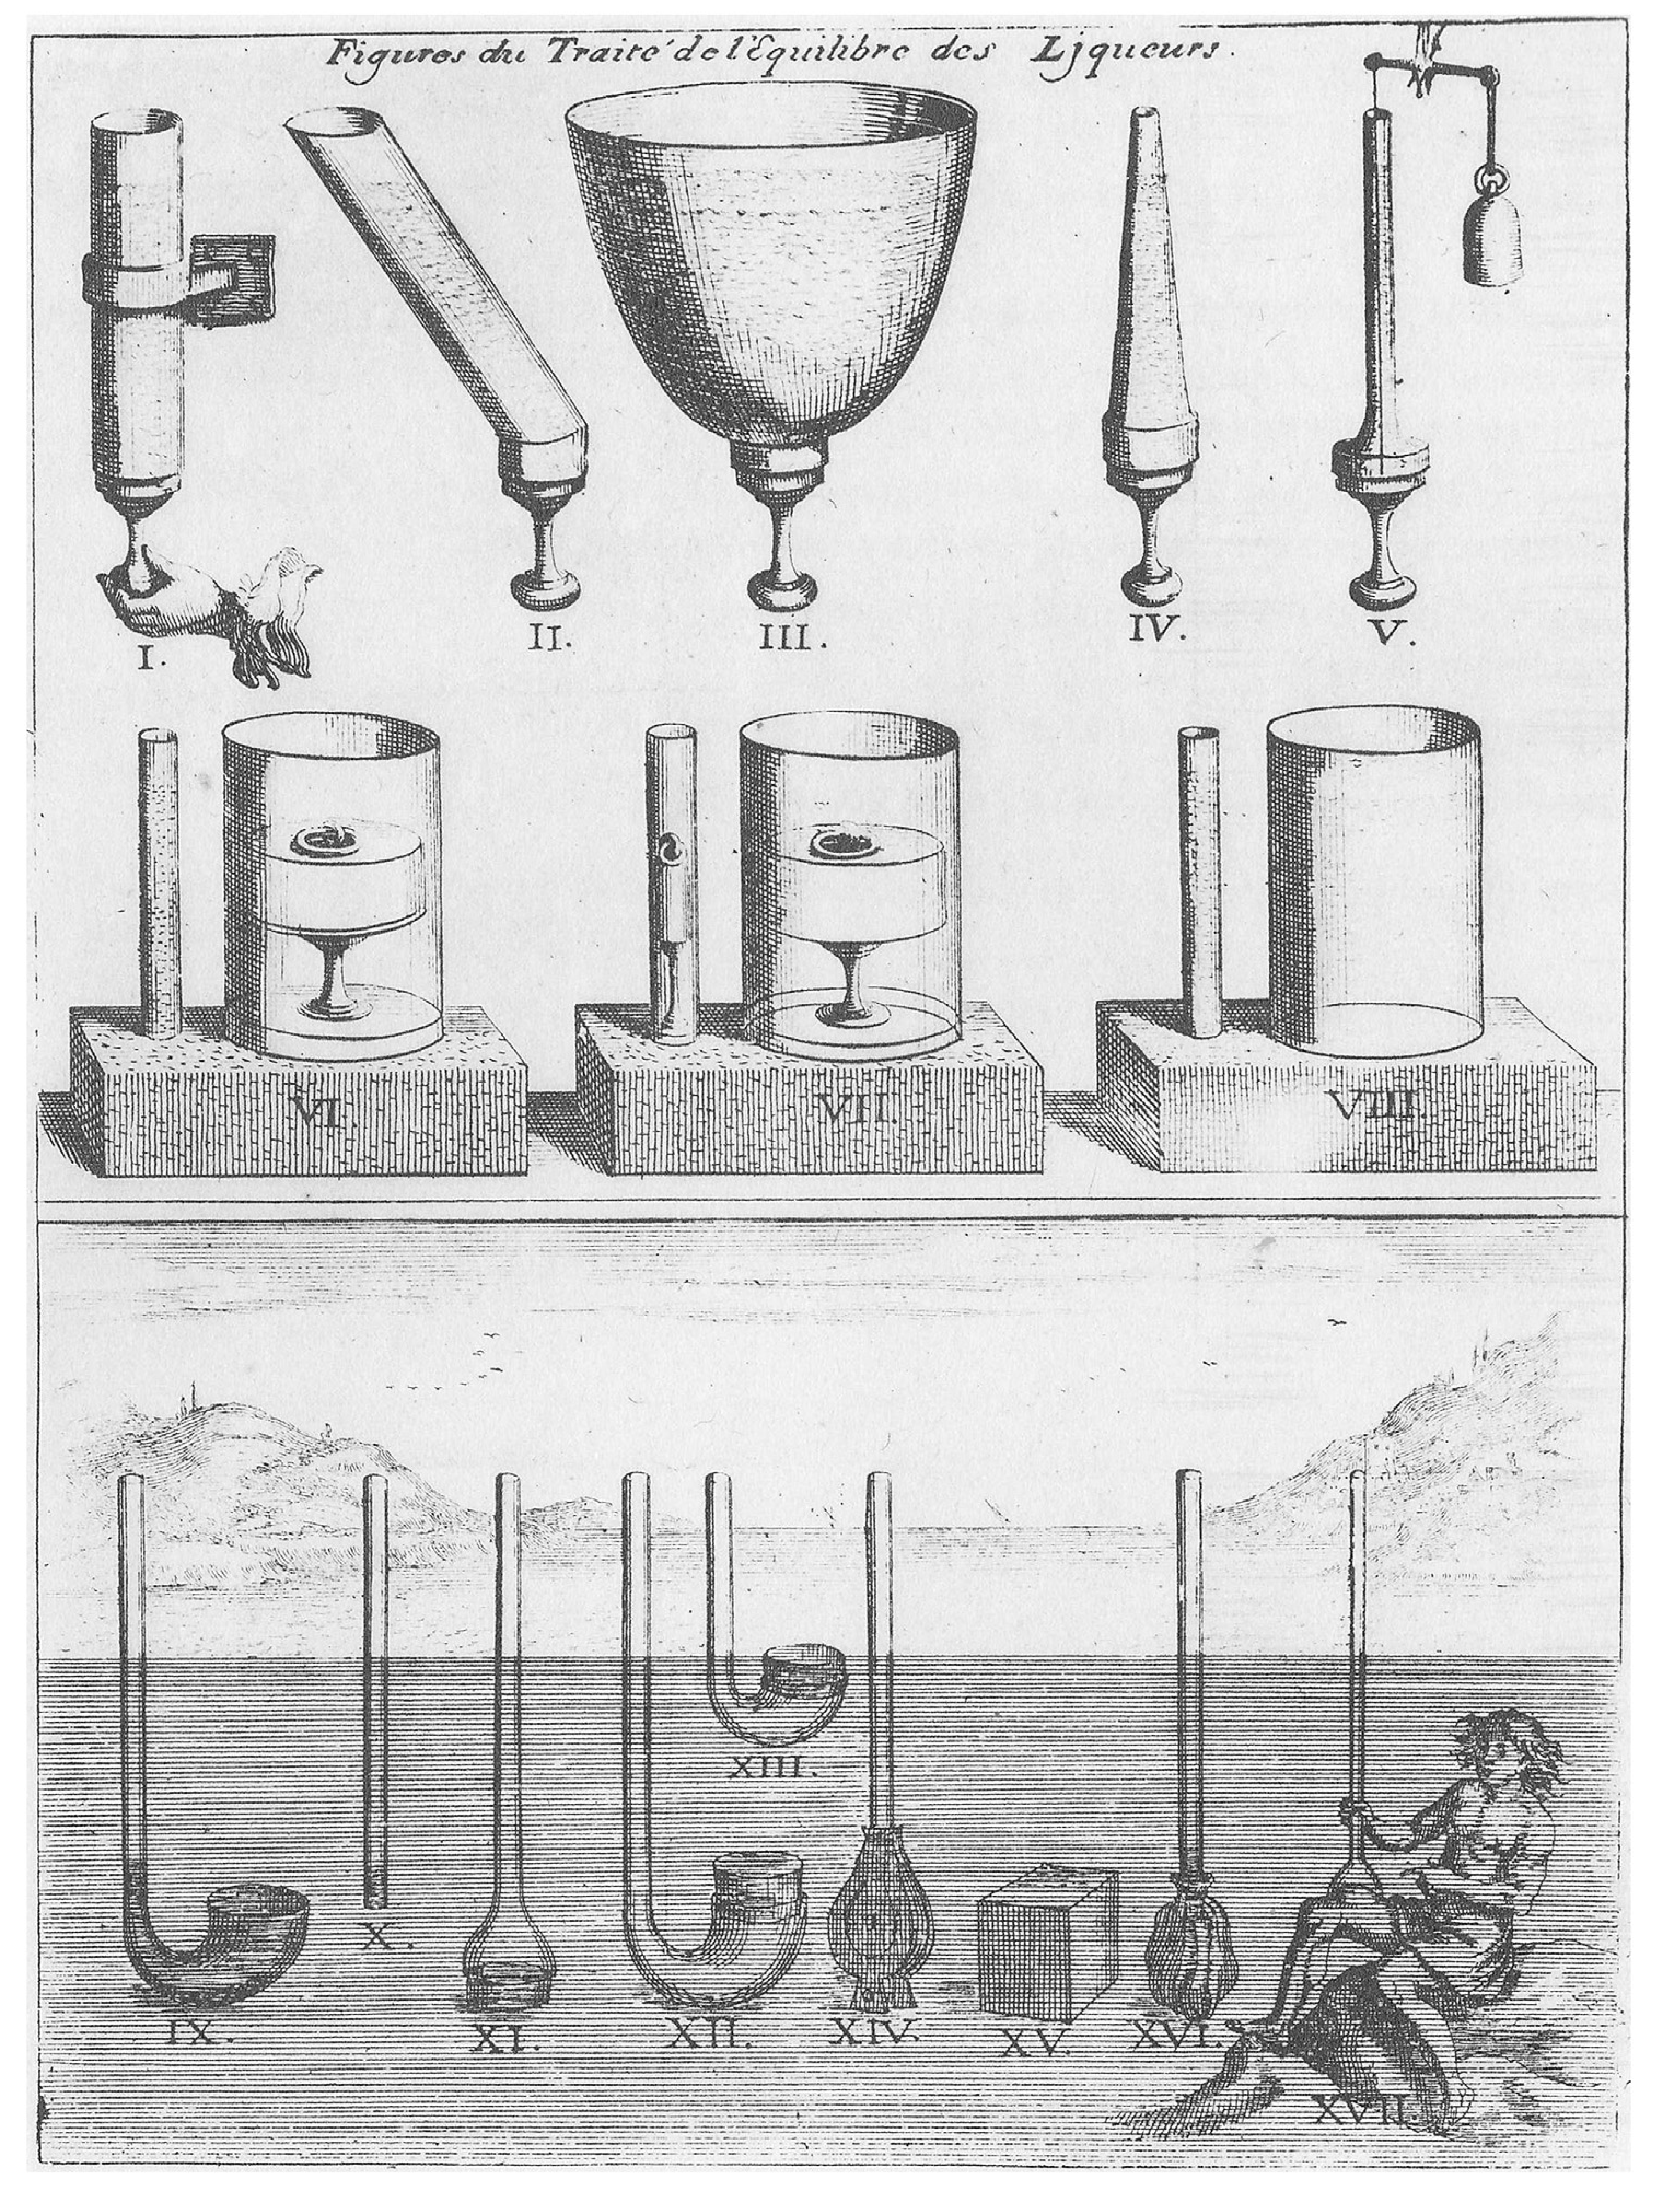
\includegraphics[width= 1\linewidth]{2}
		\caption{\small\textit{\color{cackithi}Logo của Kỳ thi toán học liên bang Đức.}}
		\vspace*{-10pt}
	\end{figure}
	Kỳ thi toán học liên bang kéo dài khoảng $14$ tháng với ba vòng thi, trong đó hai vòng thi đầu là bài tập về nhà và vòng thi cuối là thảo luận toán học. Ở mỗi vòng bài tập về nhà các thí sinh có nhiều tháng để suy nghĩ về các câu hỏi trước khi đưa ra lời giải. Ở vòng thi cuối, thí sinh sẽ có một giờ đồng hồ để thảo luận toán học với các nhà toán học. Mô hình này bị ảnh hưởng một thức tế là những vấn đề của toán học thường cần nhiều tháng đến nhiều năm để có thể có một bước tiến chứ không phải vài giờ đồng hồ. Ngoài ra, để có thể thành công trong toán học, bên cạnh kỹ năng giải toán thì kỹ năng trao đổi và truyền đạt cũng thực sự cần thiết. 
	\vskip 0.1cm
	Nội dung của kỳ thi toán học liên bang phù hợp với học sinh từ lớp $9$ đến lớp $13$. Tuy vậy, tất cả học sinh ở Đức ở mọi lứa tuổi có sự đam mê và kiên trì đều được khuyến khích tham gia. Những thí sinh đạt giải ở vòng một sẽ được mời tham gia vòng hai. Những thí sinh giành giải nhất ở vòng hai sẽ được mời tham gia vòng thảo luận toán học. Phần thưởng cho những người chiến thắng ở vòng cuối sẽ là những suất học bổng có giá trị để họ tiếp tục theo đuổi con đường học tập và nghiên cứu sau này. Ngoài ra, những thí sinh đạt giải cao ngay ở vòng hai sẽ được mời tham dự kỳ thi tuyển chọn học sinh đại diện cho nước Đức tham gia kỳ thi Olympic toán học quốc tế.
	\vskip 0.1cm
	Hiện tại kỳ thi toán học liên bang năm 2023 đang ở vòng thứ hai. Vòng thi này sẽ kết thúc vào ngày $01.09.2023$. Pi mời các độc giả cùng thử sức với đề thi năm nay nhé!
	\vskip 0.1cm
	\textbf{\color{cackithi}Vòng $\pmb{1.}$}
	\vskip 0.1cm
	\textbf{\color{cackithi}Câu $\pmb{1}$}: Ba bạn Tick, Trick và Track có $20$, $23$ và $25$ vé để đi vòng quay ngựa gỗ tại hội chợ hàng năm. Họ thống nhất rằng sẽ chỉ đi vòng quay nếu cả ba cùng đi và mỗi người nộp một vé của mình. Ngoài ra, trước mỗi lần đi, nếu muốn, họ có thể chia lại vé cho nhau bao nhiêu lần tùy thích theo quy tắc sau: Người nào có số vé chẵn thì có thể chia một nửa số vé của mình cho một trong hai người còn lại. Hỏi có thể xảy ra rằng sau một lần đi nào đó:
	\vskip 0.1cm
	$\bullet$ Đúng một người hết vé.
	\vskip 0.1cm
	$\bullet$ Đúng hai người hết vé.
	\vskip 0.1cm
	$\bullet$ Cả ba cùng hết vé. 
	\vskip 0.1cm
	\textbf{\color{cackithi}Câu $\pmb{2}$}: Tìm tất cả các bộ ba số nguyên $(x,y,z)$ thỏa mãn phương trình 
	\begin{align*}
		x^2 + y^2 + z^2 -xy-yz-zx = 3.
	\end{align*}
	\textbf{\color{cackithi}Câu $\pmb{3}$}: Cho hai hình bình hành $ABCD$ và $AECF$ có chung đường chéo $AC$, trong đó $E$ và $F$ nằm bên trong $ABCD$. Chứng minh rằng đường tròn ngoại tiếp của các tam giác $AEB$, $BFC$, $CED$ và $DFA$ giao nhau tại một điểm. 
	\vskip 0.1cm
	\textbf{\color{cackithi}Câu $\pmb{4}$}:  Cho số thực $\alpha$ với biểu diễn thập phân $\alpha = 0,a_1 a_2 a_3 \ldots$ trong đó mỗi chữ số $a_i$ là một số nguyên tố. Các chữ số sau dấu phẩy được sắp xếp dọc theo đường được tạo ra bởi các mũi tên như trong hình bên, được tưởng tượng là tiếp tục vô tận về bên phải và xuống dưới.
	\begin{figure}[H]
		\vspace*{-5pt}
		\centering
		\captionsetup{labelformat= empty, justification=centering}
		\begin{tikzpicture}[cackithi, scale=0.8]
			\draw (0,4) node {$a_1$};
			\draw (1.5,4) node {$a_2$};
			\draw (1.5,2.5) node {$a_3$};
			\draw (0,2.5) node {$a_4$};
			\draw (0,1) node {$a_5$};
			\draw (1.5,1) node {$a_6$};
			\draw (3,1) node {$a_7$};
			\draw (3,2.5) node {$a_8$};
			\draw (3,4) node {$a_9$};
			\draw (4.5,4) node {$a_{10}$};
			\draw (4.5,2.5) node {$a_{11}$};
			\draw (4.5,1) node {$a_{12}$};
			\draw (4.5,-0.5) node {$a_{13}$};
			\draw (3,-0.5) node {$a_{14}$};
			\draw (1.5,-0.5) node {$a_{15}$};
			\draw (0,-0.5) node {$a_{16}$};
			\draw (0,-2) node {$a_{17}$};
			\draw (1.5,-2) node {$a_{18}$};
			\draw (3,-2) node {$a_{19}$};
			\draw (4.5,-2) node {$a_{20}$};
			\draw (6,-2) node {$a_{21}$};
			\draw (6,-0.5) node {$a_{22}$};
			\draw (6,1) node {$a_{23}$};
			\draw (6,2.5) node {$a_{24}$};
			\draw (6,4) node {$a_{25}$};
			\draw (7.5,4) node {$a_{26}$};
			\draw (7.5,2.5) node {$a_{27}$};
			\draw (7.5,1) node {$a_{28}$};
			\draw [-stealth] (.5,4) -- (1,4);
			\draw [-stealth] (1.5,3.5) -- (1.5,3);
			\draw [-stealth] (1,2.5) -- (0.5,2.5);
			\draw [-stealth] (0,2) -- (0,1.5);
			\draw [-stealth] (0.5,1) -- (1,1);
			\draw [-stealth] (2,1) -- (2.5,1);
			\draw [-stealth] (3,1.5) -- (3,2);
			\draw [-stealth] (3,3) -- (3,3.5);
			\draw [-stealth] (3.5,4) -- (4,4);
			\draw [-stealth] (4.5,3.5) -- (4.5,3);
			\draw [-stealth] (4.5,2) -- (4.5,1.5);
			\draw [-stealth] (4.5,0.5) -- (4.5,0);
			\draw [-stealth] (4,-0.5) -- (3.5,-0.5);
			\draw [-stealth] (2.5,-0.5) -- (2,-0.5);
			\draw [-stealth] (1,-0.5) -- (0.5,-0.5);
			\draw [-stealth] (0,-1) -- (0,-1.5);
			\draw [-stealth] (0.5,-2) -- (1,-2);
			\draw [-stealth] (2,-2) -- (2.5,-2);
			\draw [-stealth] (3.5,-2) -- (4,-2);
			\draw [-stealth] (5,-2) -- (5.5,-2);
			\draw [-stealth] (6,-1.5) -- (6,-1);
			\draw [-stealth] (6,0) -- (6,0.5);
			\draw [-stealth] (6,1.5) -- (6,2);
			\draw [-stealth] (6,3) -- (6,3.5);
			\draw [-stealth] (6.5,4) -- (7,4);
			\draw [-stealth] (7.5,3.5) -- (7.5,3);
			\draw [-stealth] (7.5,2) -- (7.5,1.5);
			\draw (7.5, 0.33) node {$\vdots$};
		\end{tikzpicture}
		\vspace*{-5pt}
	\end{figure}
	Với mỗi $m \ge 1$, biểu diễn thập phân của số thực $z_m$ được cho bằng cách viết chữ số 0 trước dấu phẩy và sau dấu phẩy là các chữ số của dòng thứ $m$ (tính từ trên xuống) theo thứ tự từ trái sang phải. Tương tự, với mọi $n \ge 1$, số thực $s_n$ được thiết lập với các chữ số của cột thứ $n$ (tính từ bên trái sang) theo thự tự từ trên xuống dưới. Chẳng hạn $z_3 = 0, a_5a_6a_7a_{12}a_{23}a_{28}\ldots$ và $s_2 = 0,a_2a_3a_6a_{15}a_{18}a_{35}\ldots$. Chứng minh rằng:
	\vskip 0.1cm
	$(a)$ Nếu $\alpha$ là số hữu tỷ, thì tất cả các số $z_m$ và $s_n$ đều hữu tỷ.
	\vskip 0.1cm
	$(b)$ Điều ngược lại của khẳng định $(a)$ là sai.
	\vskip 0.1cm
	\textbf{\color{cackithi}Vòng $\pmb{2.}$}
	\vskip 0.1cm
	\textbf{\color{cackithi}Câu $\pmb{1}$}: Tìm ước chung lớn nhất của tất cả các số có dạng $p^6 - 7p^2 +6$ với $p$ chạy trên tập tất cả các số nguyên tố và $p \ge 11$.
	\vskip 0.1cm
	\textbf{\color{cackithi}Câu $\pmb{2}$}: Trên một hòn đảo địa hình đồi núi có $2023$ điểm quan sát. Từ mỗi điểm quan sát có thể nhìn thấy ít nhất $42$ điểm quan sát khác. Với hai điểm quan sát bất kỳ $X$ và $Y$, luôn tồn tại một số nguyên dương $n$ và các điểm quan sát $A_1,  A_2, \ldots, A_{n+1}$ sao cho $A_1 = X$, $A_{n+1} = Y$ và mỗi cặp điểm liền kề $A_i$ với $A_{i+1}$ có thể quan sát được lẫn nhau với $i = 1, 2, \ldots, n$. Số $n$ nhỏ nhất như vậy được gọi là khoảng cách quan sát (Sichtabstand). 
	\vskip 0.1cm
	Xác định khoảng cách quan sát lớn nhất có thể có giữa hai cặp điểm quan sát thỏa mãn những điều kiện ở trên.
	\vskip 0.1cm
	\textbf{\color{cackithi}Câu $\pmb{3}$}: Cho tam giác $AB$C với tâm đường tròn nội tiếp $I$. Gọi trung điểm của các cạnh $AC$ và $BC$ lần lượt là $M_b$ và $M_a$. Gọi giao điểm của đường thẳng $M_bI$ với đường thẳng $BC$ là $B'$ và giao điểm của đường thẳng $M_aI$ với đường thẳng $AC$ là $A'$. Biết rằng hai tam giác $ABC$ và $A'B'C$ có cùng diện tích. 
	\vskip 0.1cm
	Tìm giá trị lớn nhất có thể của góc $ACB$.
	\vskip 0.1cm
	\textbf{\color{cackithi}Câu $\pmb{4}$}: Cho một đa diện đều $2n$ cạnh. Từ các đoạn thẳng nối các đỉnh của đa diện (cạnh biên hoặc đường chéo) ta tô $n$ cạnh màu đỏ sao cho:
	\vskip 0.1cm
	$1.$ Các điểm cuối của các cạnh màu đỏ chính là $2n$ đỉnh của đa diện.
	\vskip 0.1cm
	$2.$  Không có $2$ cạnh màu đỏ nào có độ dài bằng nhau.
	\vskip 0.1cm
	Tìm tất cả các số tự nhiên $n \ge 2$ thỏa mãn yêu cầu đã cho.
\end{multicols}